In diesem Kapitel werden die aufgenommenen Messungen ausgewertet und deren Bedeutung graphisch analysiert. Hierbei werden die Aufnahmen von zwei dimensionalen Ausgaben, welche das Gleichgewicht des Roboters widerspiegeln und die Werte der Aktoren in den Gelenken unterschieden.

\subsection{Gleichgewichtssensoren}

Wie in Kapitel \ref{software} beschrieben, werden zwei dimensionale Ausgaben, wie die x- und y-Ausgabe des Gyroskops, in einem Scatterhistogramm dargestellt, welches es ermöglicht, die Dichteverteilung einzusehen. 

\begin{figure}[b!]
	\centering
	\begin{adjustwidth}{-0.2\linewidth}{-0.2\linewidth}
		\hspace{+35pt}
		\begin{subfigure}[c]{.5\linewidth}
			\centering
			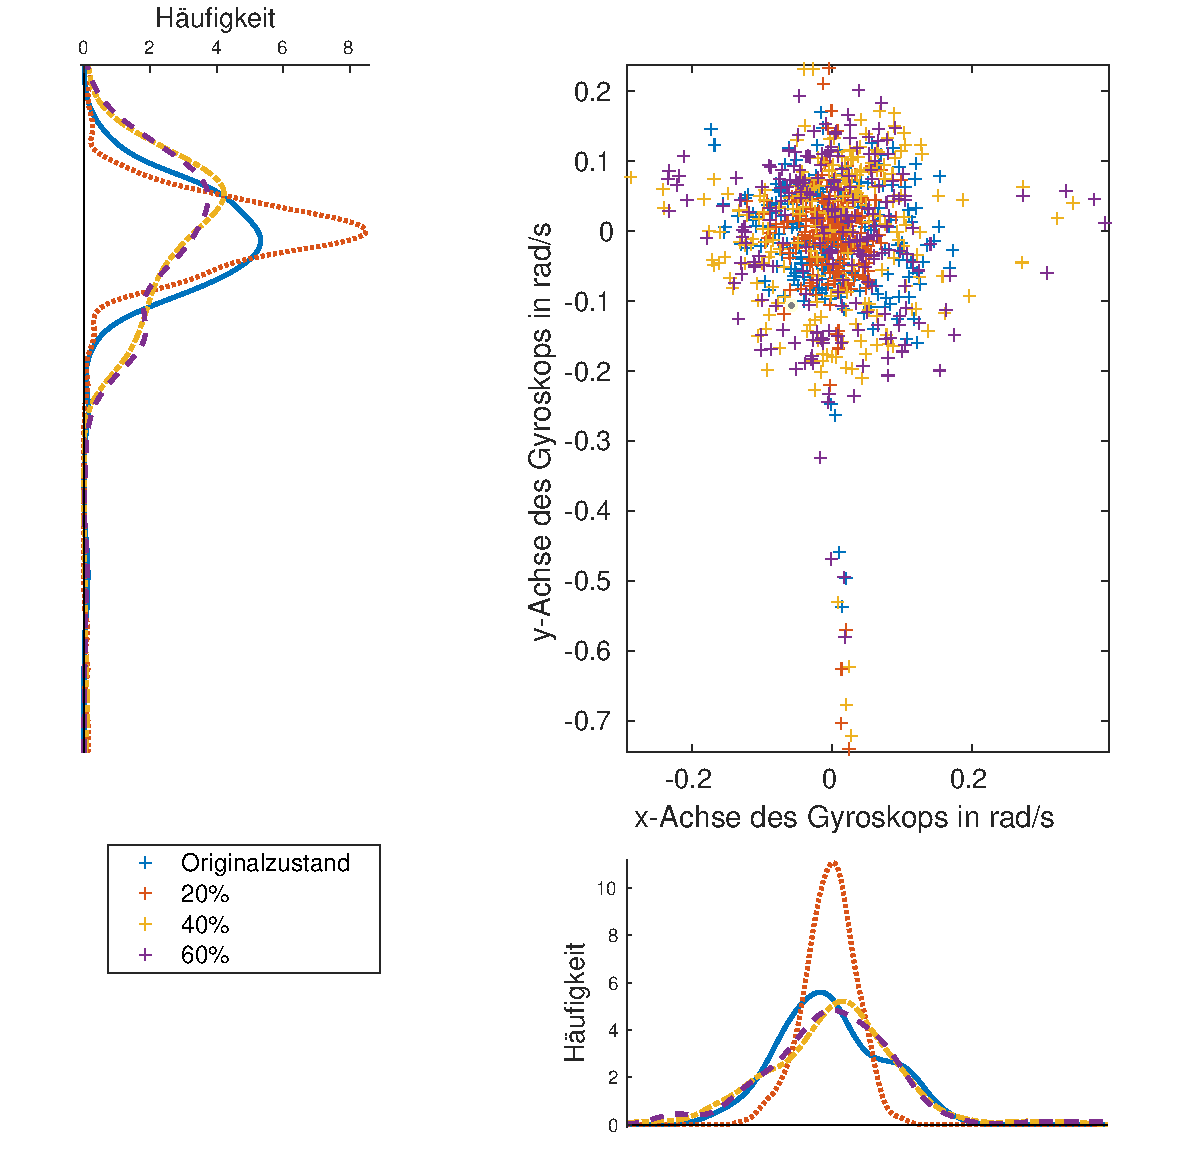
\includegraphics[width=\linewidth]{Bilder/Gyr_Grund_20_40_60_ohneM.pdf}
			\vspace{5pt}
		\end{subfigure}
		\hspace{-35pt}
		\begin{subfigure}[c]{.5\linewidth}
			\centering
			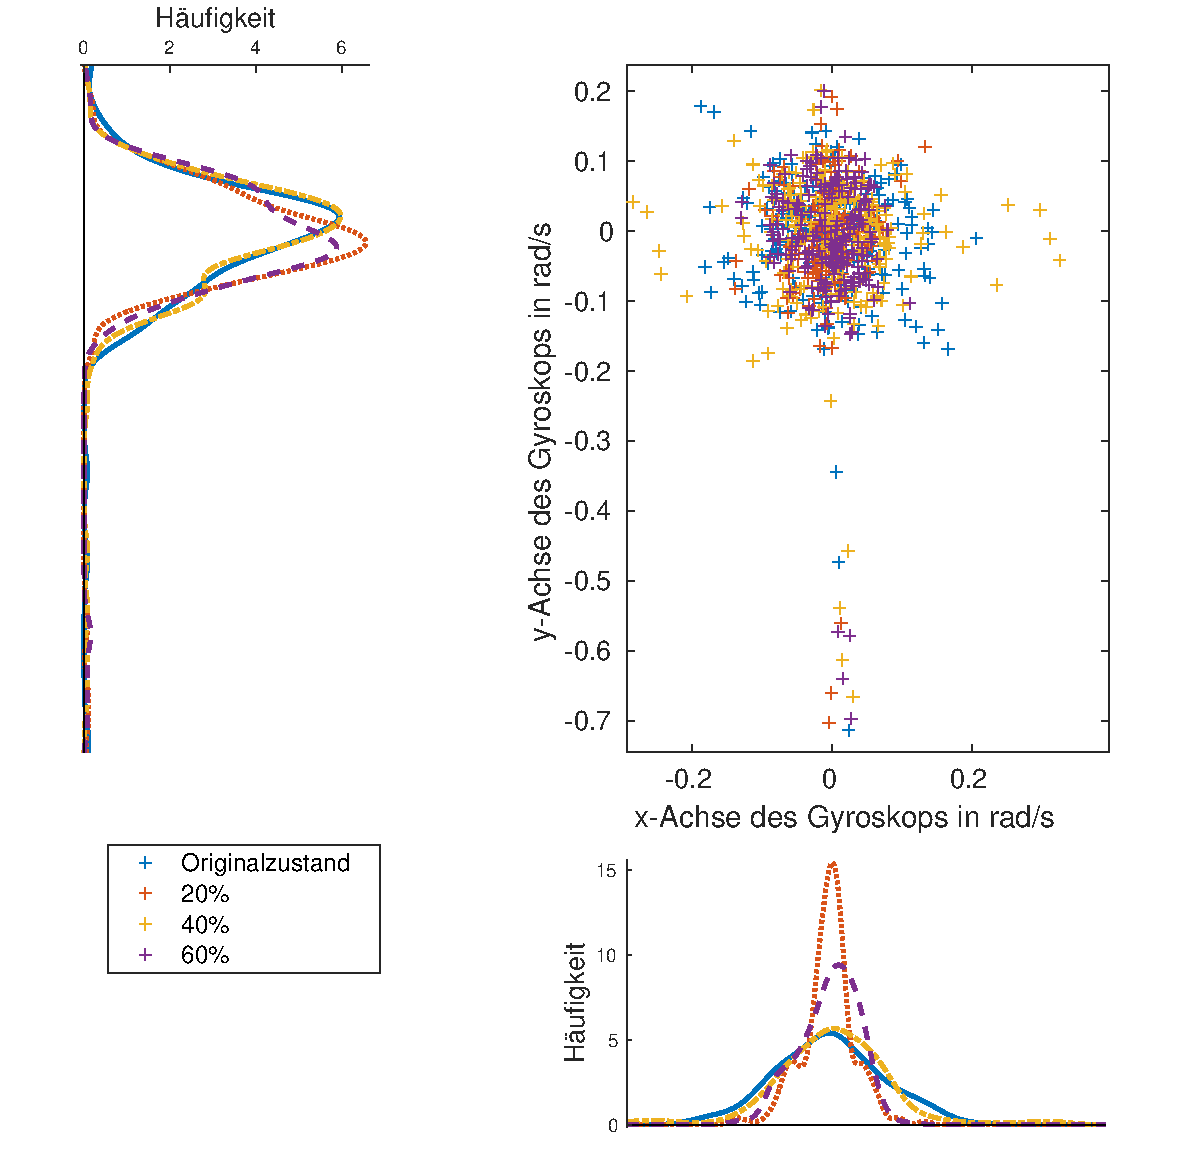
\includegraphics[width=\linewidth]{Bilder/Gyr_Grund_20_40_60_mitM.pdf}
			\vspace{5pt}
		\end{subfigure}
	\end{adjustwidth}
	\caption{Ausgabe des Gyroskops, x-Achse auf y-Achse, links ohne Magneten, rechts mit Magneten}\label{Gyr}
\end{figure}

In Abb. \ref{Gyr} sind die Aufnahmen des Gyroskops zu erkennen. Jede Ausgabe besteht aus 220 Punkten, da dies die Anzahl der Messdurchläufe pro Lauf sind. Jeder Wert wurde durch das arithmetische Mittel aus Gleichung \eqref{mean} aller Messpunkte zu diesem Zeitpunkt ermittelt. Der Graph auf der linken Seite ist die Ausgabe für die Messungen ohne Magneten an der Rampenunterseite, auf der rechten Seite die für die Messungen mit Magneten. Die jeweils zwei errechneten Dichteverteilung am linken und am unteren Rand des Hauptplots spiegeln die Verteilung des Scatterplots eindimensional wider. Die vereinzelten Punkte unterhalb von $-0,3 \unit{rad/s}$ sind dem Beginn der Messung geschuldet, während derer NAO sich in aufrechtem Stand befindet. Sobald der Roboter die laufende Haltung einnimmt, wird der Torso deshalb relativ schnell bewegt. Dies wird während der restlichen Aufnahmen nur passieren, wenn NAO umfällt. 
%Sollte ich hierfür das Gyroskop einmal auf die Zeit gesehen zeigen?

% abb 13: wie sind die Graphen aufgeteilt, was haben die Graphen an der seite zu bedeuten. Warum sind da vereinzelnd punkte in der mitte unten

Bei einem stabilen Gang würde man erwarten, dass die Geschwindigkeit, in der sich der Torso bewegt, gering bleibt. Dies bedeutet, je mehr Ausschwankungen zu sehen sind, desto instabiler läuft dieser Roboter und desto eher würde er das Gleichgewicht verlieren. 
% was würde man erwarten, wenn NAO stabil läuft

In Abb. \ref{Gyr} ist eine Tendenz von stabiler werdendem Gang von ohne Magneten zu mit Magneten zu erkennen. Allerdings fällt dies auch für den Originalschuh auf, welcher kein MAP enthält. Grund hierfür könnte der etwa 1cm breite Magnet sein, welcher den unteren Teil des Schuhs in Stellung hält, bevor die Schrauben zur Befestigung verwendet werden.

Des Weiteren heben sich die Sohlen mit $20\,\%$ CIP Anteil besonders hervor. Durch die Magneten erfahren sie ebenfalls eine minimale Verbesserung. Hierbei sollte erwähnt werden, dass diese Sohle mit der gedruckten Halterung dem Gewicht der Originalsohle am nächsten kommt und dadurch die Stabilität vielleicht besser gewährleistet ist. Die stärkste Auswirkung sowohl für die x- als auch die y-Achse gab es für $60\,\%$ CIP Anteil. Dies ist nicht verwunderlich, da hier die größte magnetische Kraft wirkt. 
% erst dann: man sieht eine Tendenz, dass es mit Magneten stabiler ist. 20% ist von vorn herein sehr stabil, der Grundschuh sowie 40% zeigen zeigt in y-Achse eine starke verbesserung mit Magneten, 60% zeigt in allen Achsen eine Verbesserung der Stabilität

\begin{figure}[htb]
	\centering
	\begin{adjustwidth}{-0.2\linewidth}{-0.2\linewidth}
		\hspace{+45pt}
		\begin{subfigure}[c]{.45\linewidth}
			\centering
			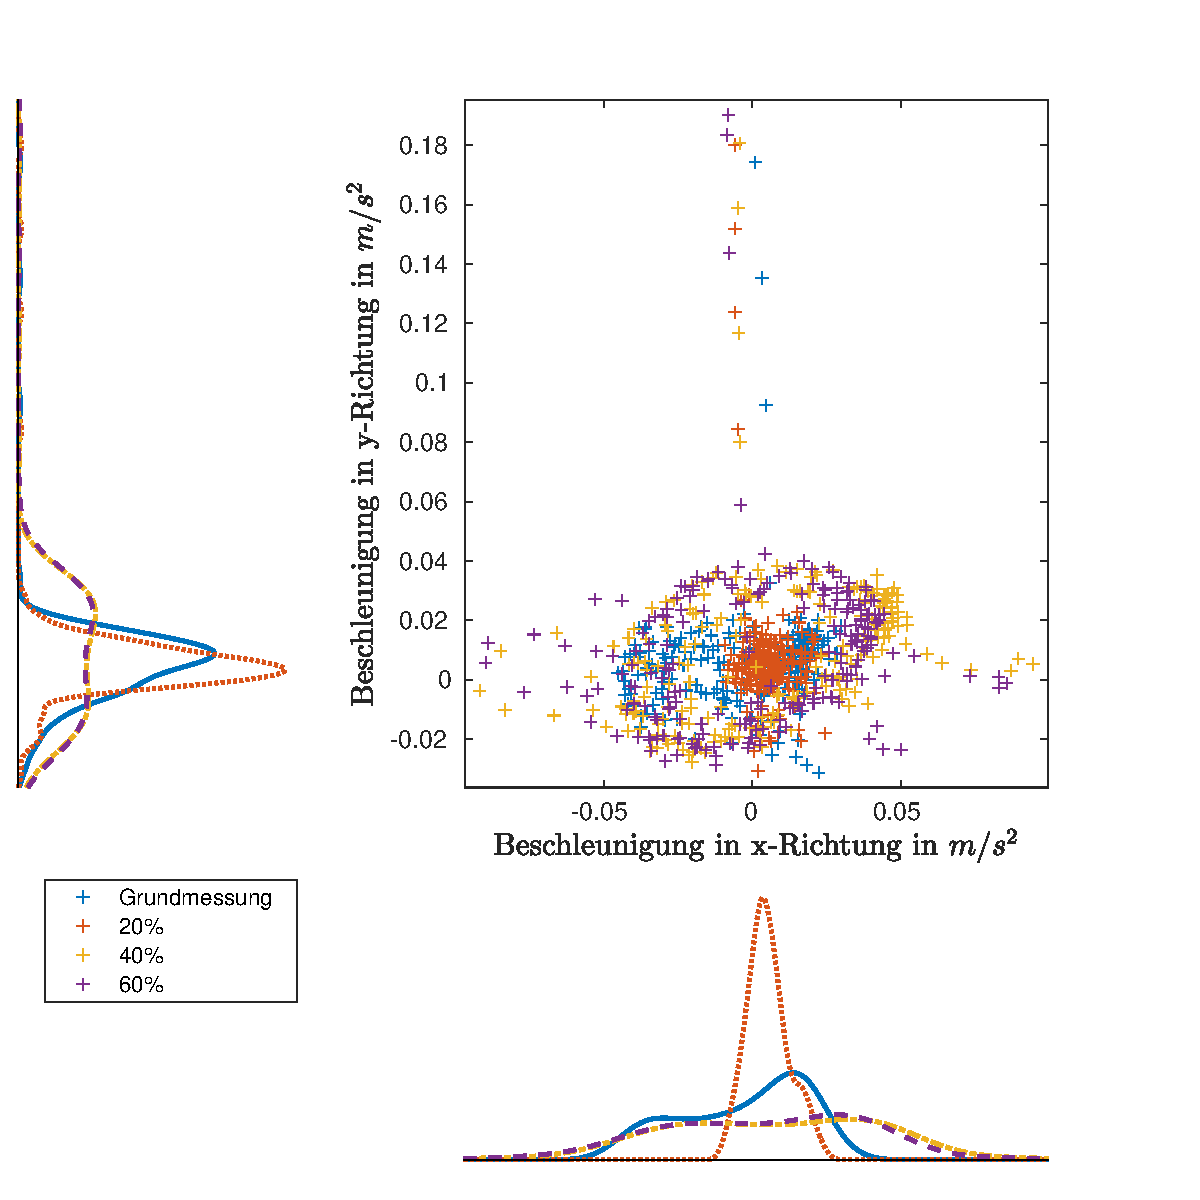
\includegraphics[width=\linewidth]{Bilder/Beschleunigung_Grund_20_40_60_ohneM.pdf}
			\vspace{5pt}
		\end{subfigure}
		%\hfill
		\hspace{-25pt}
		\begin{subfigure}[c]{.45\linewidth}
			\centering
			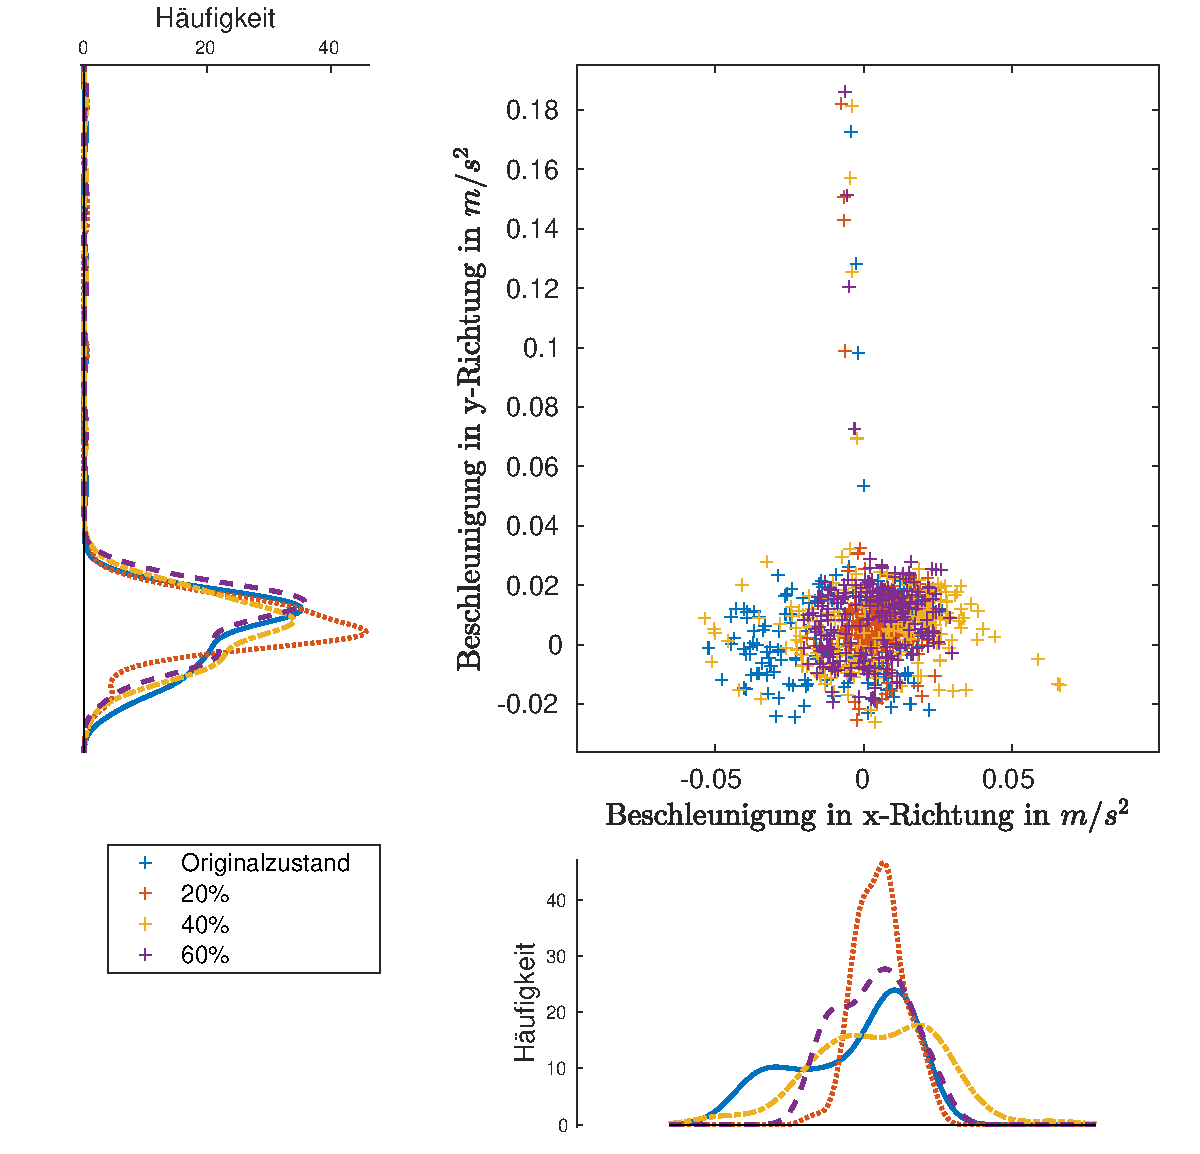
\includegraphics[width=\linewidth]{Bilder/Beschleunigung_Grund_20_40_60_mitM.pdf}
			\vspace{5pt}
		\end{subfigure}
	\end{adjustwidth}
	\caption{Ausgabe des Beschleunigungssensors, x-Achse auf y-Achse aufgetragen, links ohne Magneten, rechts mit Magneten} \label{Acc}
\end{figure}
Die Beschleunigungssensoren messen wie bereits erwähnt in $\unit{m/s^2}$ die Beschleunigung des Torsos. Deshalb ist ebenfalls zu erwarten, dass bei einem stabilen Gang diese Werte sich in der Nähe des Nullpunkts zentrieren, sollte NAO stabil laufen. Genau wie in Abb. \ref{Gyr} zeigen die Graphen in Abb. \ref{Acc} eine Tendenz zu einem stabileren Lauf mit Magneten. Auch hier wirken die $20\,\%$igen Proben außergewöhnlich stabil, während die $60\,\%$igen Proben in x-Richtung von den Magneten am meisten Profitieren. Gleichzeitig verhalten sich $40$ zu $60\,\%$ in y-Richtung ähnlich. 
% abb 14: Gleiche Graphenaufteilung, ähnliches Ergebnis

\begin{figure}[tb]
	\centering
	\begin{adjustwidth}{-0.2\linewidth}{-0.2\linewidth}
		\hspace{45pt}
		\begin{subfigure}[c]{.45\linewidth}
			\centering
			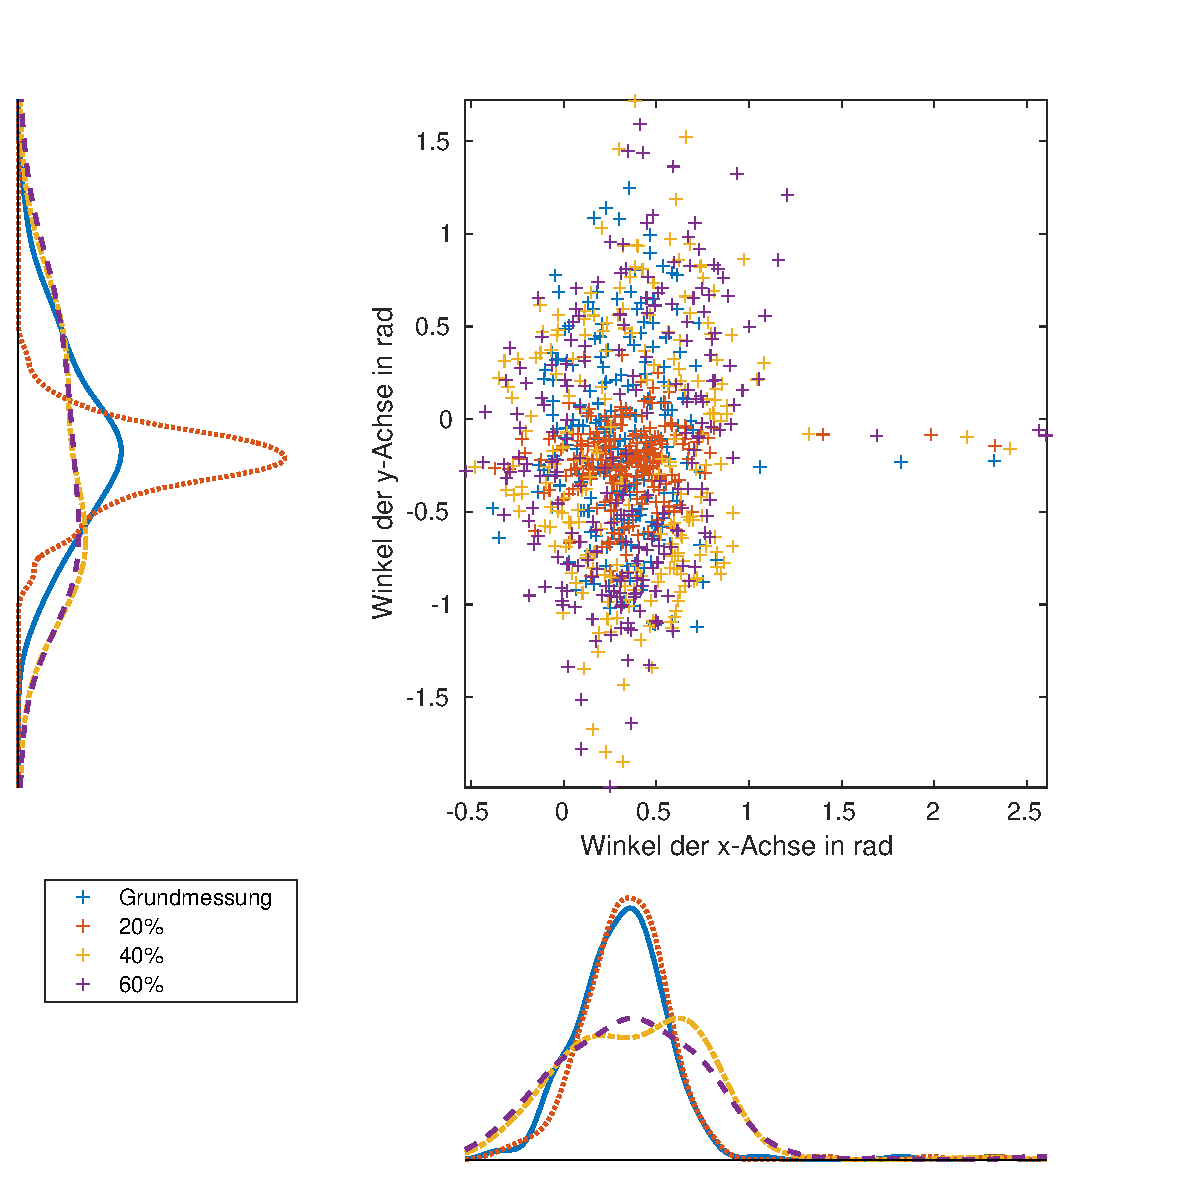
\includegraphics[width=\linewidth]{Bilder/Winkel_Grund_20_40_60_ohneM.pdf}
			\vspace{5pt}
		\end{subfigure}
		\hspace{-20pt}
		%\hfill
		\begin{subfigure}[c]{.45\linewidth}
			\centering
			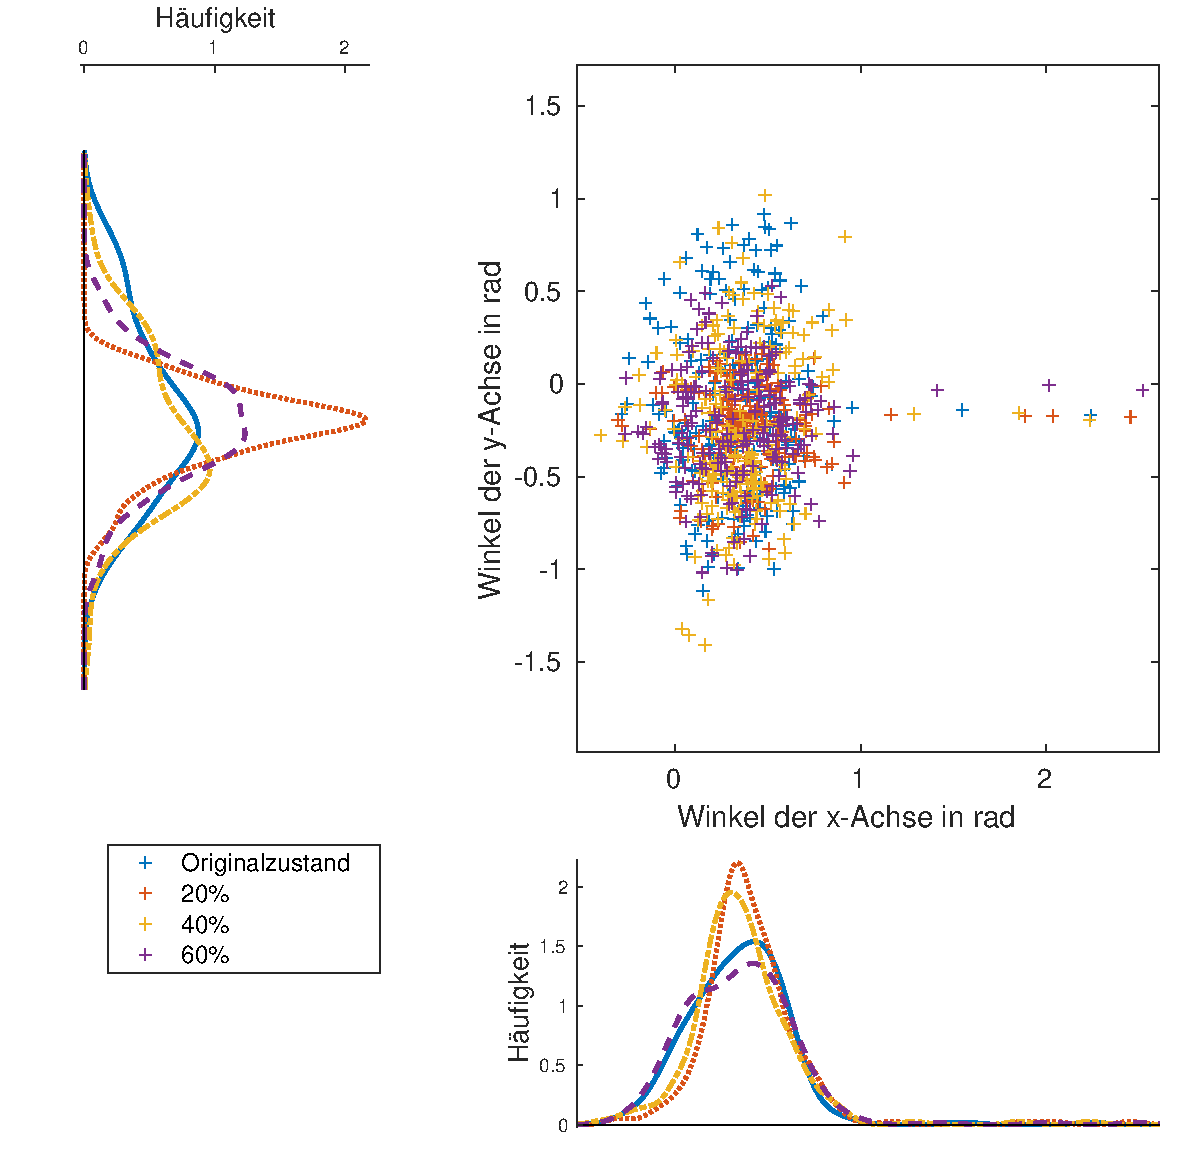
\includegraphics[width=\linewidth]{Bilder/Winkel_Grund_20_40_60_mitM.pdf}
			\vspace{5pt}
		\end{subfigure}
	\end{adjustwidth}
	\caption{Echtzeit errechneter Winkel, x-Achse auf y-Achse aufgetragen, links ohne Magneten, rechts mit Magneten} \label{Angle}
\end{figure}
Die Winkelwerte in Abb. \ref{Angle} entstehen aus der Berechnung durch Gyroskop und Beschleunigungssensor. Da beide alle Graphen zuvor eine Tendenz von höherer Stabilität durch Magneten aufwiesen, ist zu erwarten, dass dies bei den Winkelgraphen auch der Fall ist. In der y-Achse ist eine Verbesserung von $40$ und $60\,\%$ erkennbar.In x-Richtung scheint $40\,\%$iges MAP am meisten zu profitieren, allerdings gilt für den Originalschuh eher das Gegenteil. 
% abb 15: Ist aus den Werten, welche in abb 13 und 14 zu sehen sind errechnet. deshalb auch hier ähnliches Ergebnis

\begin{figure}[tb]
	\centering
	\begin{adjustwidth}{-0.2\linewidth}{-0.2\linewidth}
		\hspace{40pt}
		\begin{subfigure}[c]{.45\linewidth}
			\centering
			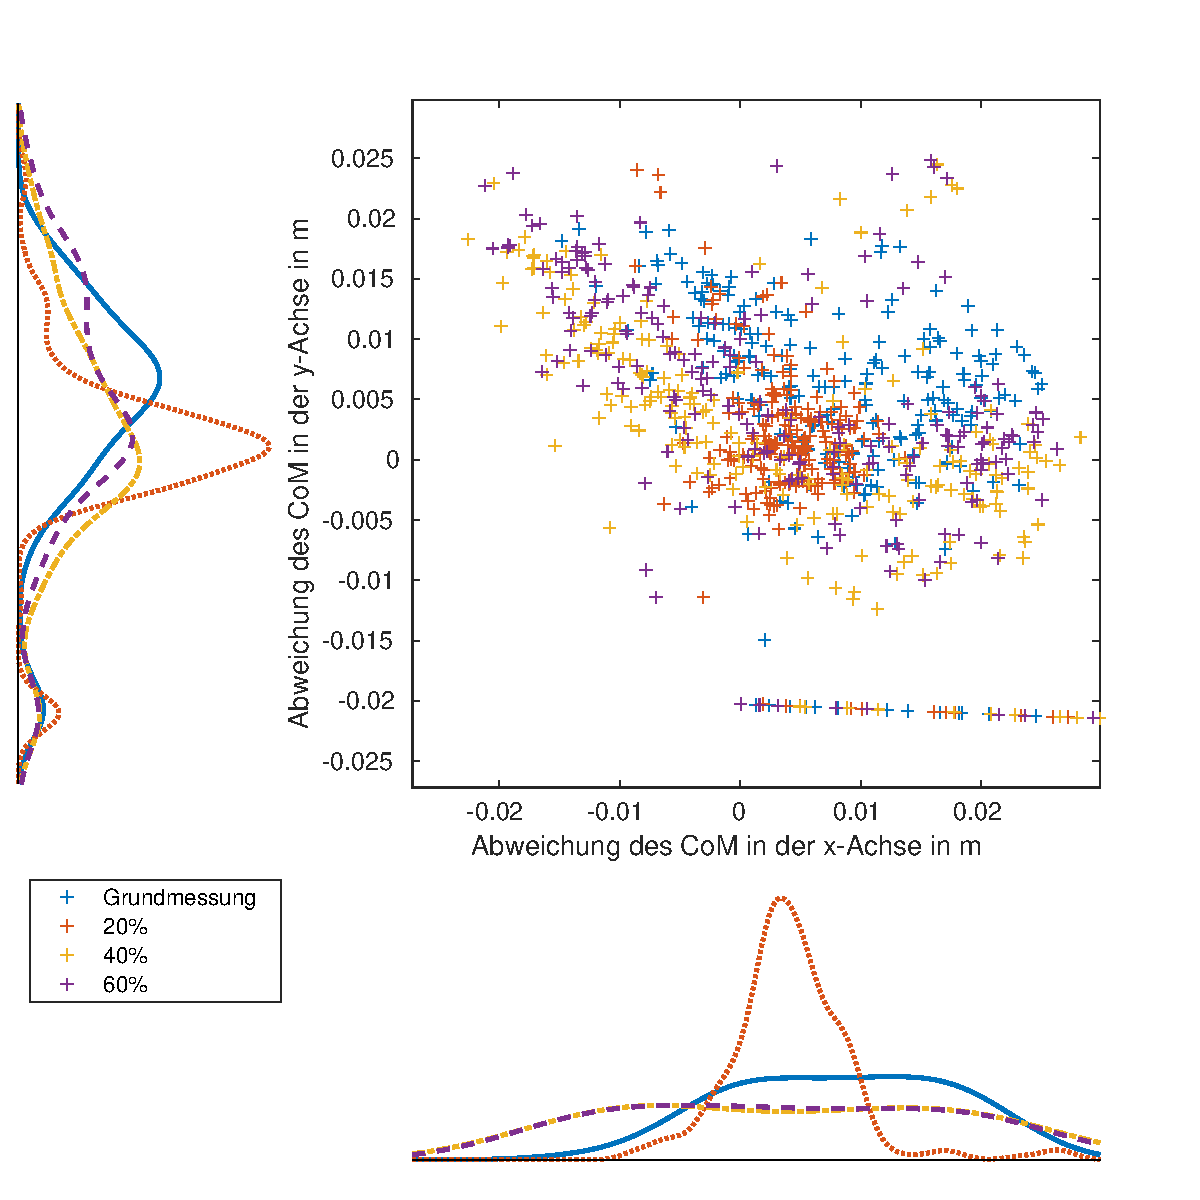
\includegraphics[width=\linewidth]{Bilder/links_CoM_ohneM.pdf}
			\vspace{5pt}
		\end{subfigure}
		\hspace{-10pt}
		%\hfill
		\begin{subfigure}[c]{.45\linewidth}
			\centering
			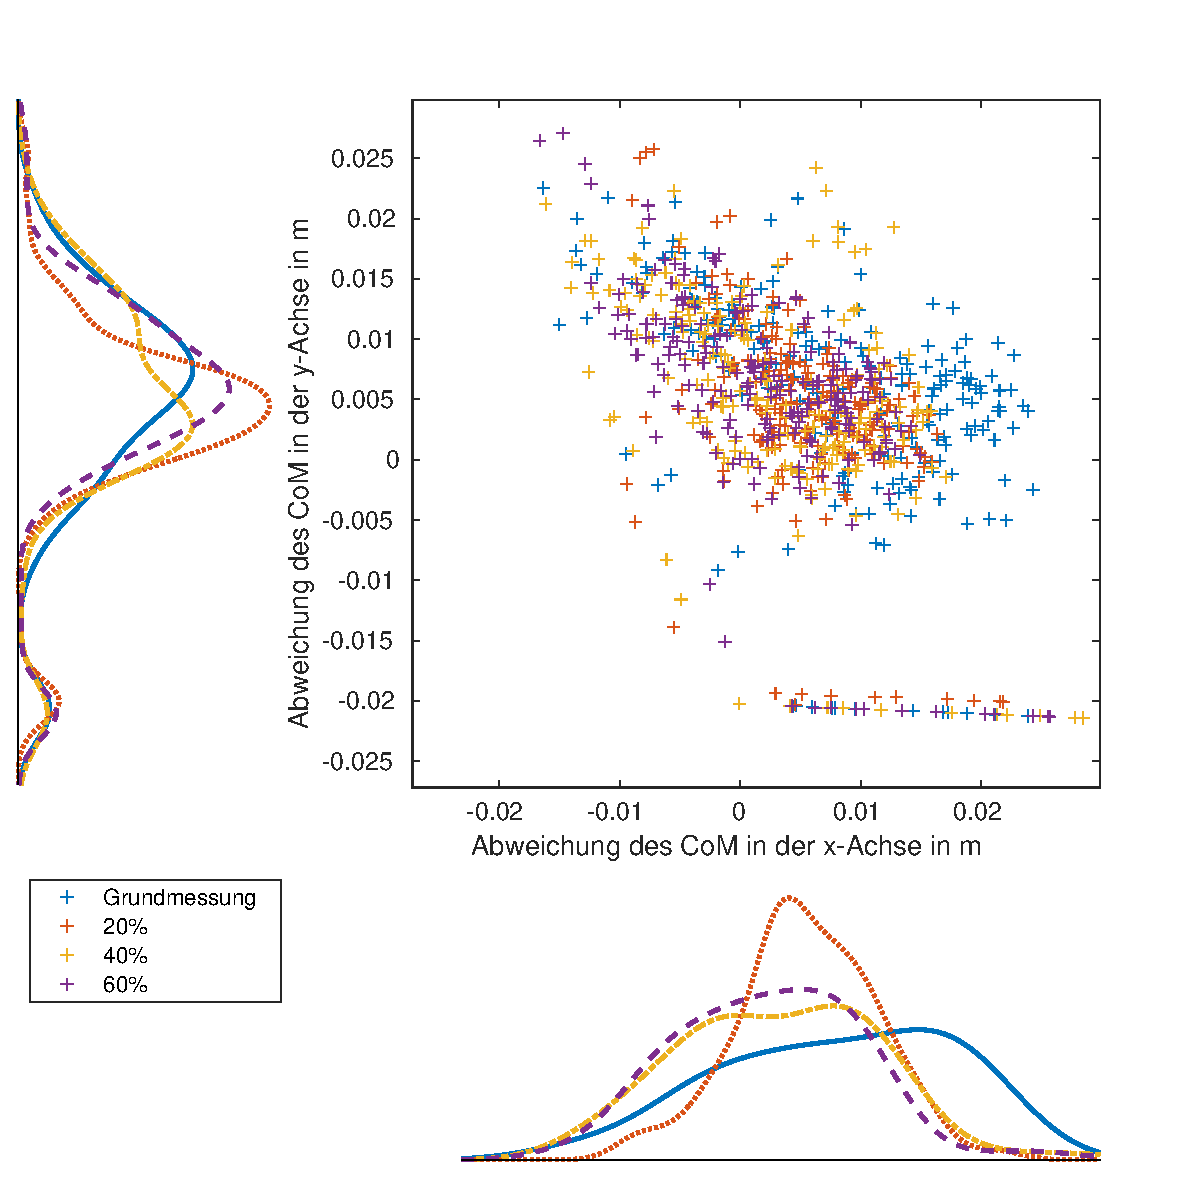
\includegraphics[width=\linewidth]{Bilder/links_CoM_mitM.pdf}
			\vspace{5pt}
		\end{subfigure}
	\end{adjustwidth}
	\caption{Linker errechneter Massenschwerpunkt aufgenommen durch die FSR, x-Achse auf y-Achse aufgetragen, links ohne Magneten, rechts mit Magneten} \label{CoM_links}
\end{figure}
\begin{figure}[tb]
	\centering
	\begin{adjustwidth}{-0.2\linewidth}{-0.2\linewidth}
		\hspace{40pt}
		\begin{subfigure}[c]{.45\linewidth}
			\centering
			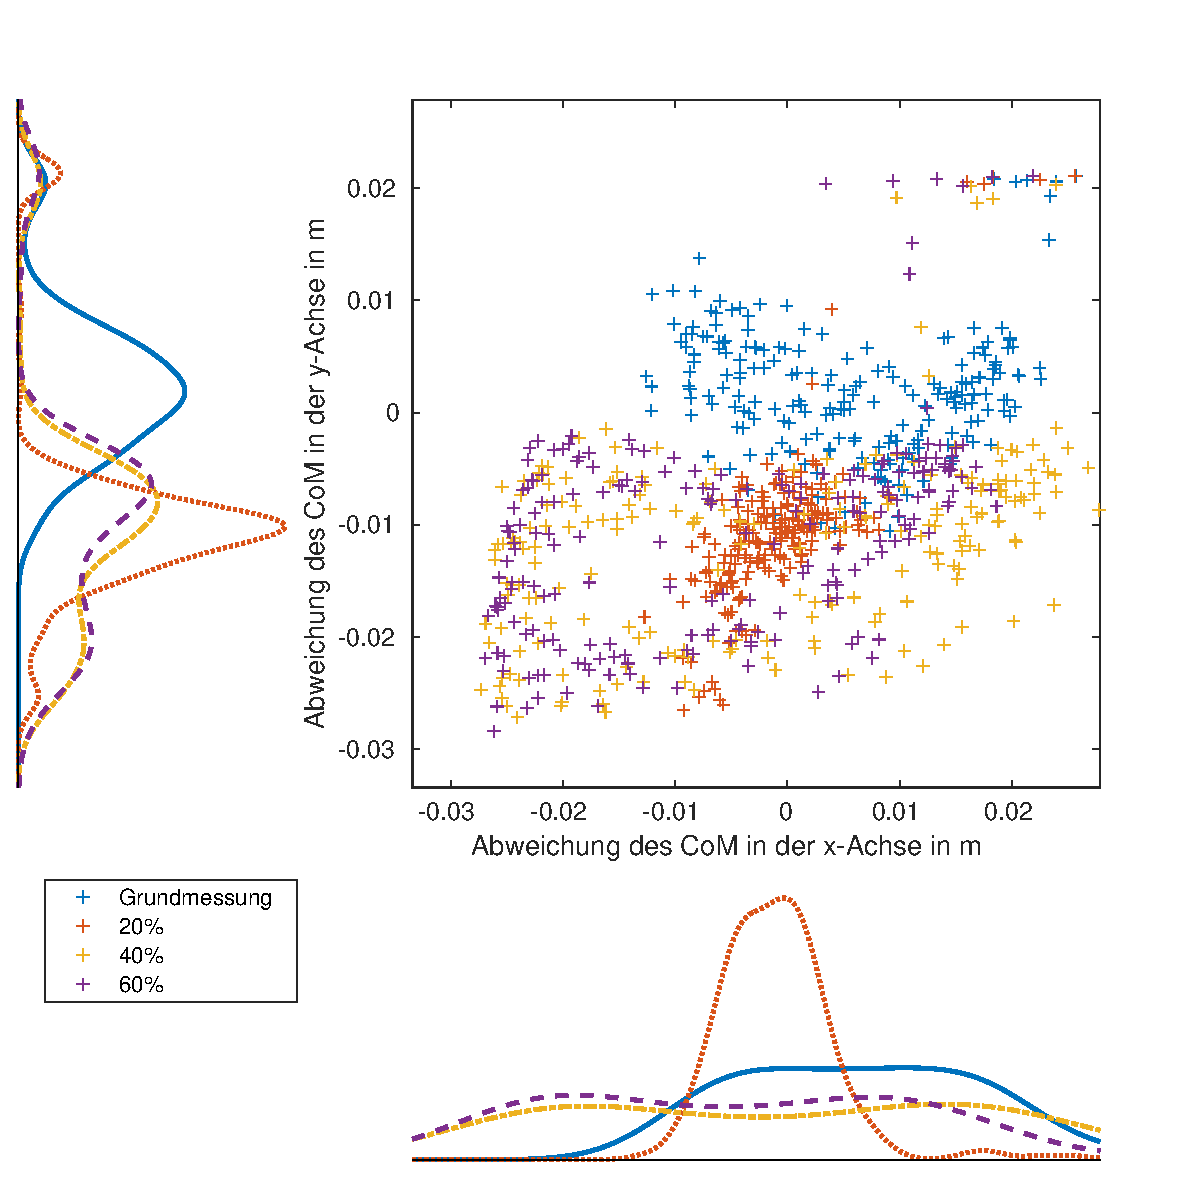
\includegraphics[width=\linewidth]{Bilder/rechts_CoM_ohneM.pdf}
			\vspace{5pt}
		\end{subfigure}
		\hspace{-10pt}
		%\hfill
		\begin{subfigure}[c]{.45\linewidth}
			\centering
			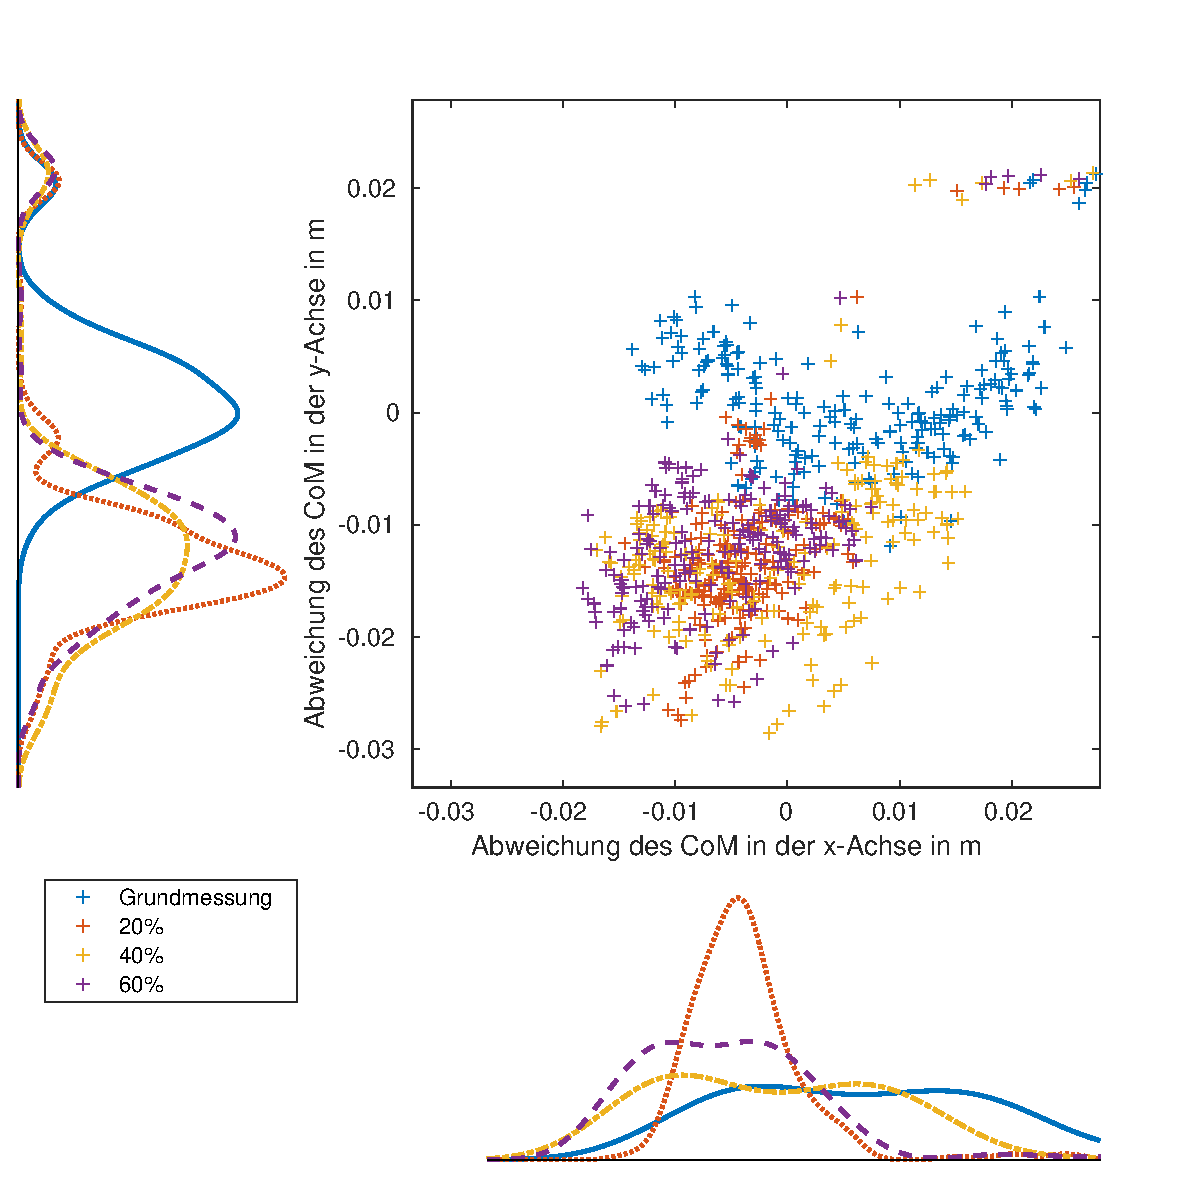
\includegraphics[width=\linewidth]{Bilder/rechts_CoM_mitM.pdf}
			\vspace{5pt}
		\end{subfigure}
	\end{adjustwidth}
	\caption{Rechter errechneter Massenschwerpunkt aufgenommen durch die FSR, x-Achse auf y-Achse aufgetragen, links ohne Magneten, rechts mit Magneten} \label{CoM_rechts}
\end{figure}
Das hier verwendete Modell von NAO bietet die Möglichkeit die Stabilität des Gangs über die in Kapitel \ref{aufbau_NAO} erwähnten Drucksensoren in den Fußsohlen zu messen. Die errechneten Werte der zweidimensionalen Massenschwerpunkte durch die 8 FSR Sensoren sind in Abb \ref{CoM_links} und \ref{CoM_rechts} zu sehen. Auf einer Zeitskala aufgetragen lässt sich erkennen, dass zu Beginn der Messaufzeichnungen einige y-Werte sich in der Nähe von $-0,02$ bzw. $0,02$ aufhalten. Dies geschieht während des Gangs allerdings nicht, daher entsteht bei allen Aufnahmen ein zu vernachlässigender Sammelbereich im rechten unteren Bereich bei Abb. \ref{CoM_links} und im rechten oberen Bereich von Abb. \ref{CoM_rechts}. 

In beiden Abbildungen ist wie bei den bisherigen Graphen die erhöhte Stabilität mit Magneten sichtbar. Die Werte liegen konzentrierter um einen Punkt. Hier ist der Unterschied zwischen dem Originalschuh größer, denn wie in Abb. \ref{total_weight} gezeigt, vermessen die FSR weniger mit den MAP Sohlen, die größte Differenz ist in Abb. \ref{CoM_rechts} zu sehen, bei der das Maximum der Dichteverteilung der y-Achse deutlich weiter links liegt. Auf der x-Achse ist zu vermerken, dass der Originalschuh durch das Magnetfeld eher an Stabilität verliert, während alle anderen Sohlen der Stabilität zuträglich sind.  
% abb 16 und 17 sind aus den FSR Daten entstanden und weißen eine ebenfalls weisen nur für die MAP sohlen unterschiede auf, aber kaum für den Grundschuh. 

In allen Graphen ist ersichtlich, dass die Probeläufe mit $20\,\%$ CIP in der MAP Sohle ungewöhnlich stabil sind, was auf einen Zufall hindeuten könnte. Denn insgesamt gab es zwei Fehlschläge bei denen NAO das Gleichgewicht verloren hat, einmal mit $20\,\%$ und einmal mit $40\,\%$, beides mit Magneten an der Rampe. Außerdem wurde bei früheren Messungen eine erhöhte Stabilität bei $40\,\%$ im Vergleich zu anderen Proben und dem Grundschuh festgestellt. Dies lässt darauf schließen, dass für eine Sicherstellung der Unterschiede zwischen den einzelnen Proben deutlich mehr Testläufe erforderlich sind. Dennoch lässt sich abschließend sagen, dass ein stabilerer Lauf durch die Magneten erzielen wurde. Die größte Auswirkung hatten die Magneten wie zu erwarten war auf die Proben mit einem höheren CIP Anteil. Gleichzeitig sind diese Sohlen allerdings bis zu doppelt so schwer wie der Originalschuh, siehe Tabelle \ref{gewicht}. 

% Warum diese Auswertung mit Vorsicht zu genießen ist: frühere Auswertung
% Ungenauigkeiten der FSR
% Dennoch wird bei allen Graphen eine verbesserung mit Magneten festgestellt, warum könnte das so sein?


%Notizen:
%
%Die folgenden Graphen unterscheiden sich in ihrer Darstellung: Zum einen wurden Gyroskop, Beschleunigungssensors, Winkel und Center of Mass in sog. Scatterhistogrammen geplottet, siehe Abb \ref{Gyr},\ref{Acc},\ref{Angle}. Der Hauptplot ist ein scatter-Plot, welcher die Verteilung auf der X verglichen zur Y-Achse zeigt. An den Rändern sind jeweils die Histogramme der Achsen aufgetragen, welche die Wahrscheinlichkeitsverteilung angeben. Dabei ist die Annahme, dass ein stabilierer Gang eine steilere Wahrscheinlichkeitsverteilung hervorbringt, da sich die Aufnahmepunkte in der Mitte häufen müssten. Eine flache Verteilungskurve würde im Gegenzug bedeuten, dass NAO während dem Gang große Schwankungen aufweist und deshalb instabiler läuft.
%
%Es lässt sich eine Tendenz erkennen, dass der Gang mit Magneten stabiler ist, als ohne. Außerdem zeichnet sich das 20\,\% MAP durch besonders gute Stabilität hab. 
%
%Der Strom wurde in Histogrammen aufgetragen, welche die relative Häufigkeit des Stroms während der Messung aufzeigt. Die Graphen \ref{AnklePitch_Current_links},\ref{AnklePitch_Current_rechts},\ref{AnkleRoll_Current_links},\ref{AnkleRoll_Current_rechts} sind unterteilt in zwei Arten von Plots. Einerseits ist ein Histogramm mit jeweils 20 Säulen zu sehen. Diese wurde mit der Wahrscheinlichkeitsdichtefunktion von Matlab (pdf) ergänzt, um die Verteilung besser einsehen zu können.
%
%Die Annahme ist, dass ein höherer Strom mehr Reibungs- oder Haftwiderstand bedeuten. Leider ist die Datenlage hier sehr uneindeutig. 

\FloatBarrier
\subsection{Sensoren der Aktoren}

\begin{figure}[tb]
	\centering
%	\begin{adjustwidth}{-0.2\linewidth}{-0.2\linewidth}
%		\hspace{5pt}
		\begin{subfigure}[c]{.9\linewidth}
			\centering
			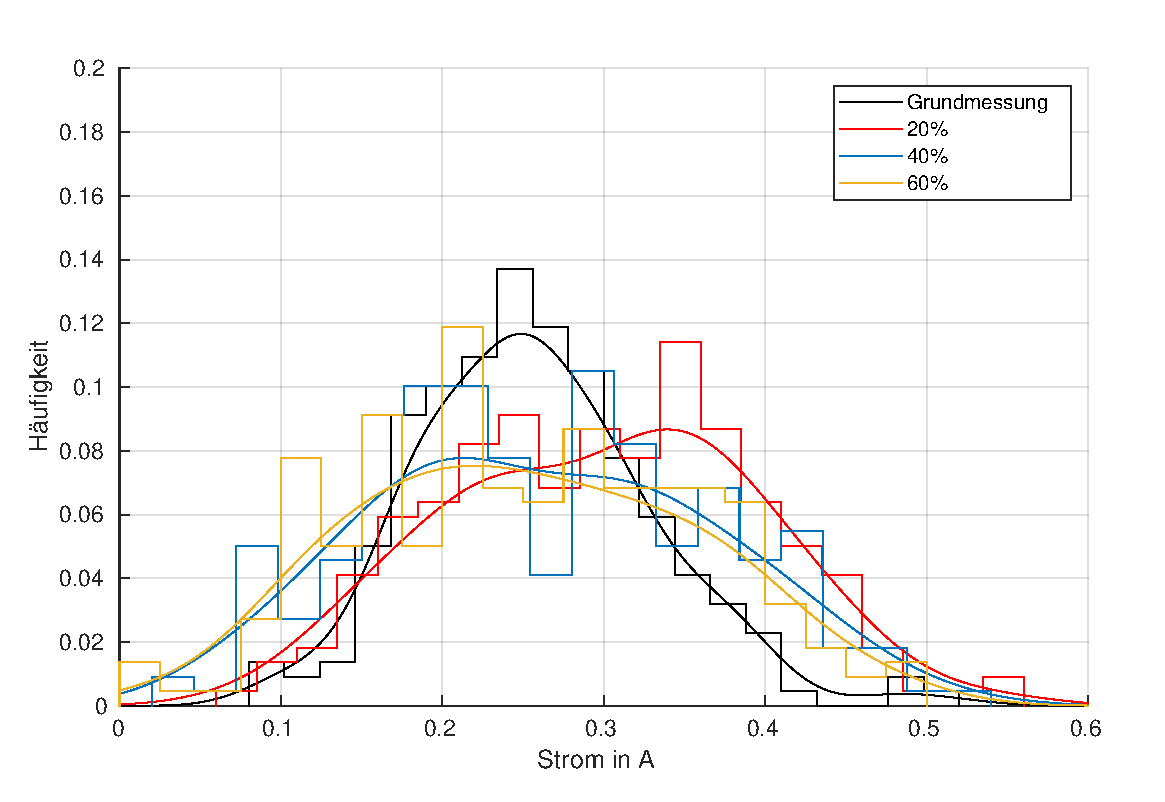
\includegraphics[width=\linewidth]{Bilder/links_Current_AnklePitch_ohneM.pdf}
%			\vspace{5pt}
		\end{subfigure}
%		\hspace{20pt}
%		\hfill
		\begin{subfigure}[c]{.9\linewidth}
			\centering
			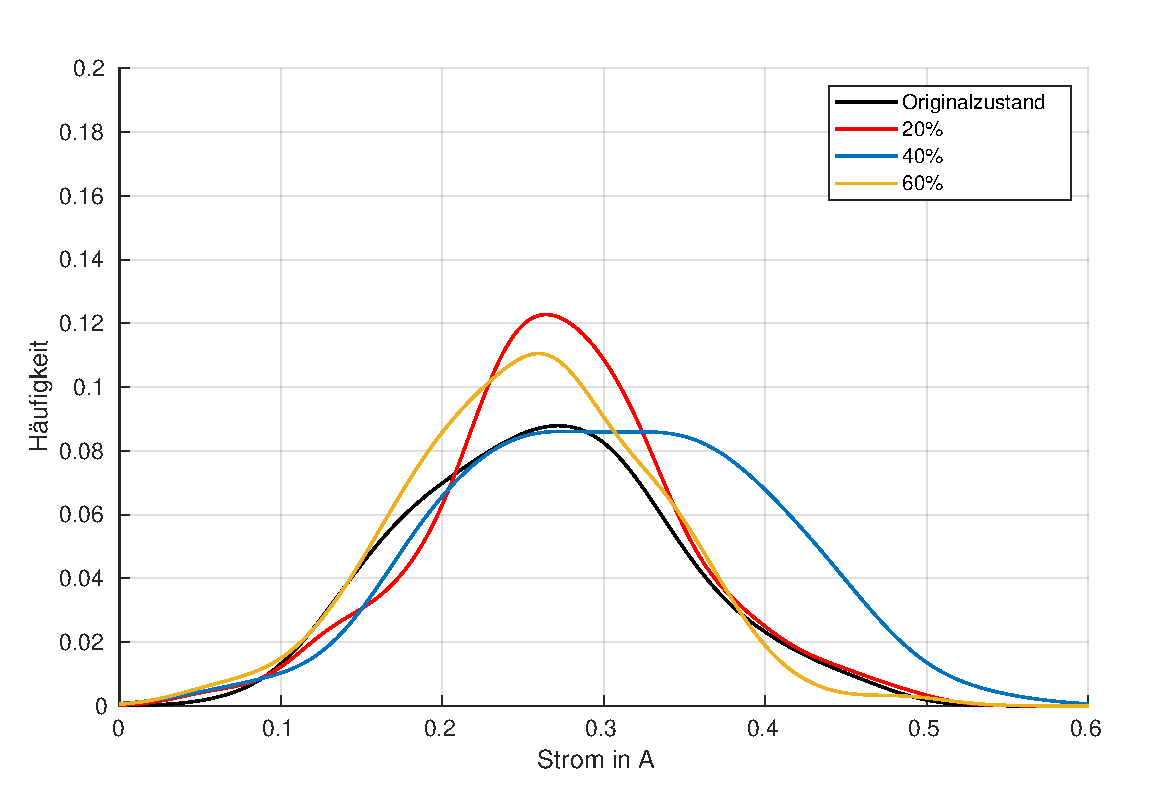
\includegraphics[width=\linewidth]{Bilder/links_Current_AnklePitch_mitM.pdf}
%			\vspace{5pt}
		\end{subfigure}
%	\end{adjustwidth}
	\caption{AnklePitch gemessener Strom im linken Fuß, Strom in Ampère aufgetragen auf die Häufigkeit. Das Histogramm wurde ergänzt durch eine Wahrscheinlichkeitsdichtefunktion. Der obere Graph sind die Aufnahmen ohne Magneten, der untere mit Magneten.} \label{AnklePitch_Current_links}
\end{figure}
\begin{figure}[tb]
	\centering
%	\begin{adjustwidth}{-0.2\linewidth}{-0.2\linewidth}
%		\hspace{5pt}
		\begin{subfigure}[c]{.9\linewidth}
			\centering
			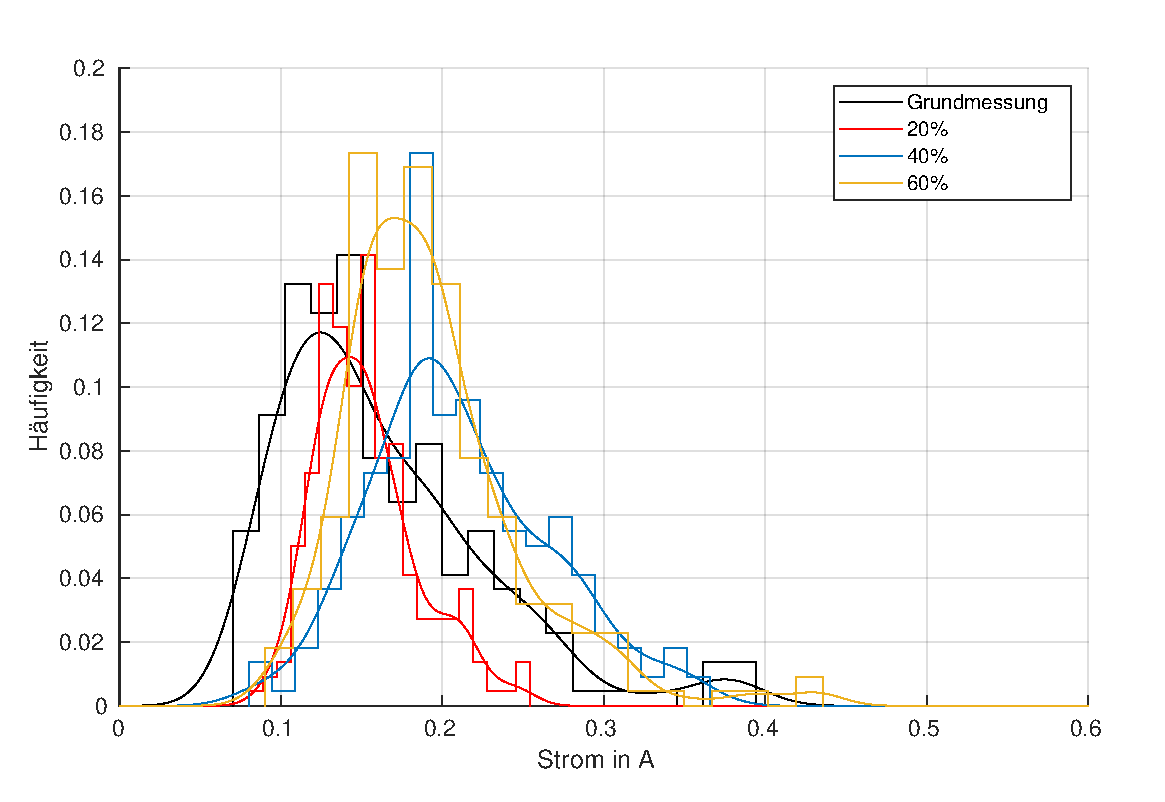
\includegraphics[width=\linewidth]{Bilder/rechts_Current_AnklePitch_ohneM.pdf}
			\vspace{5pt}
		\end{subfigure}
%		\hspace{20pt}
		\hfill
		\begin{subfigure}[c]{.9\linewidth}
			\centering
			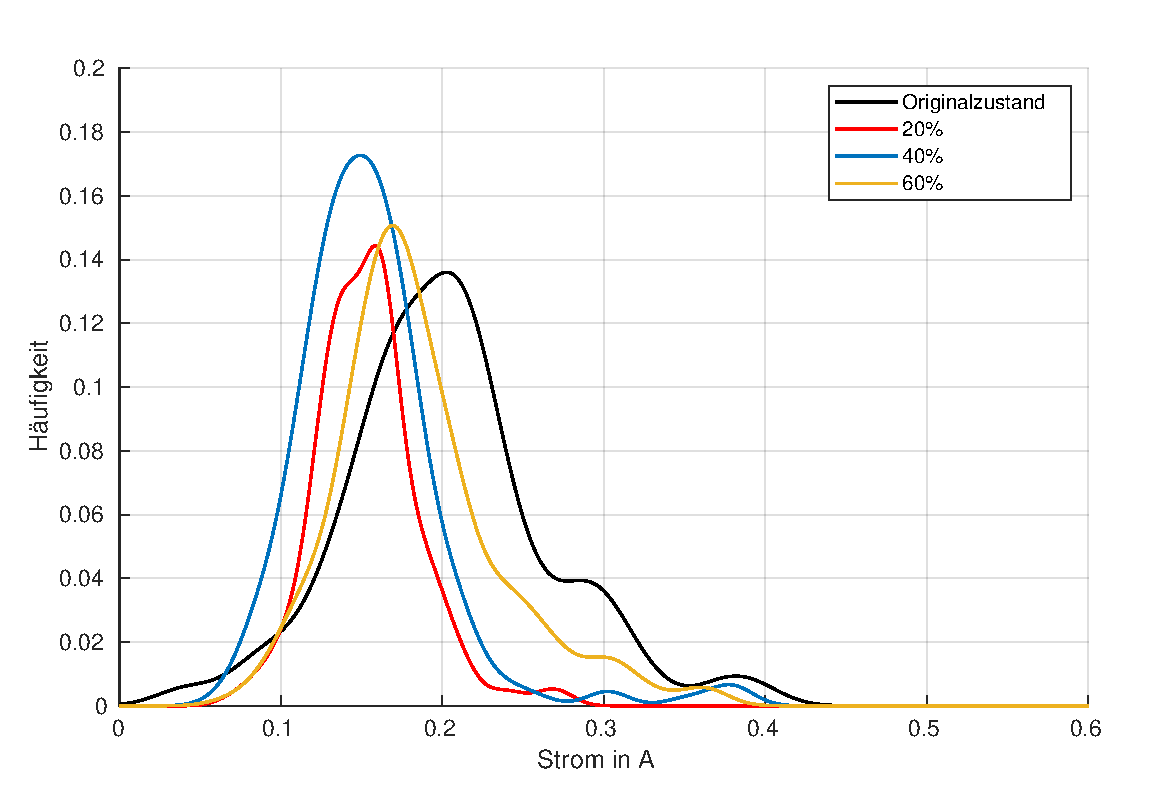
\includegraphics[width=\linewidth]{Bilder/rechts_Current_AnklePitch_mitM.pdf}
			\vspace{5pt}
		\end{subfigure}
%	\end{adjustwidth}
	\caption{AnklePitch gemessener Strom im rechter Fuß, Strom in Ampère aufgetragen auf die Häufigkeit. Das Histogramm wurde ergänzt durch eine Wahrscheinlichkeitsdichtefunktion. Der obere Graph sind die Aufnahmen ohne Magneten, der untere mit Magneten.} \label{AnklePitch_Current_rechts}
\end{figure}

\begin{figure}[tb]
	\centering
	%	\begin{adjustwidth}{-0.2\linewidth}{-0.2\linewidth}
	%		\hspace{5pt}
	\begin{subfigure}[c]{.9\linewidth}
		\centering
		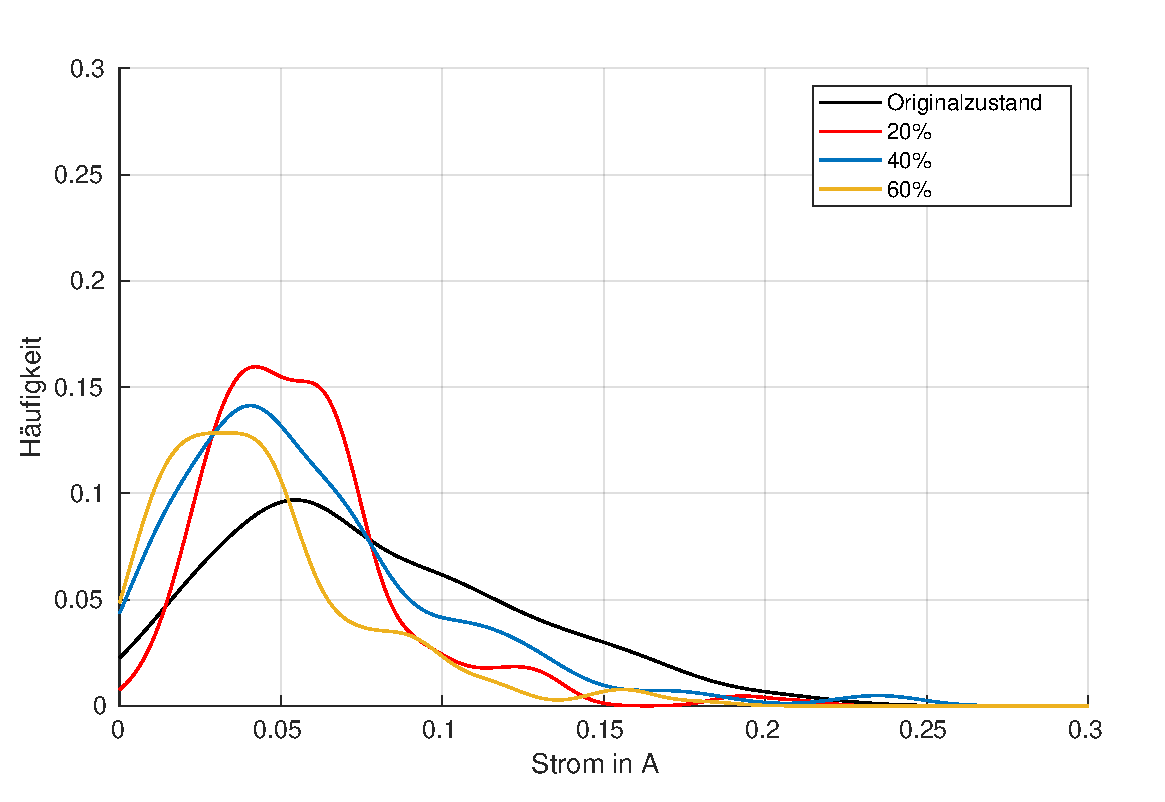
\includegraphics[width=\linewidth]{Bilder/links_Current_AnkleRoll_ohneM.pdf}
		%			\vspace{5pt}
	\end{subfigure}
	%		\hspace{20pt}
	%		\hfill
	\begin{subfigure}[c]{.9\linewidth}
		\centering
		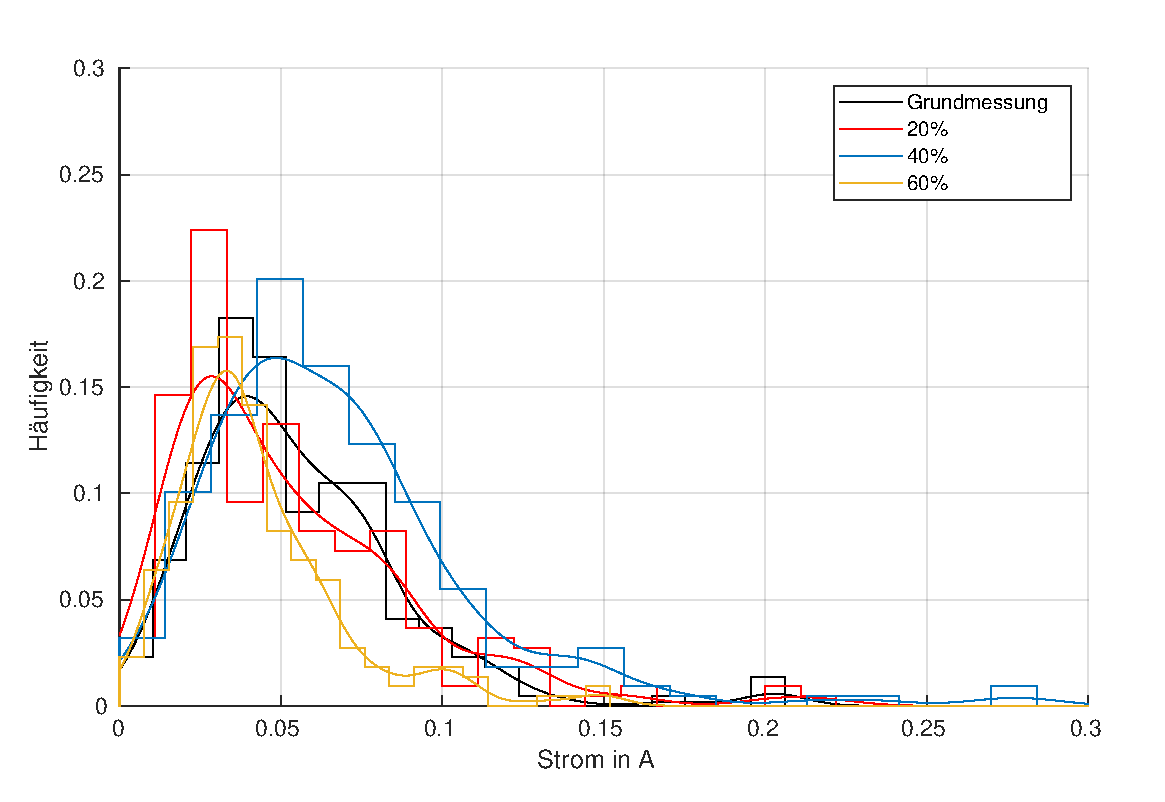
\includegraphics[width=\linewidth]{Bilder/links_Current_AnkleRoll_mitM.pdf}
		%			\vspace{5pt}
	\end{subfigure}
	%	\end{adjustwidth}
	\caption{AnkleRoll gemessener Strom im linken Fuß, Strom in Ampère aufgetragen auf die Häufigkeit. Das Histogramm wurde ergänzt durch eine Wahrscheinlichkeitsdichtefunktion. Der obere Graph sind die Aufnahmen ohne Magneten, der untere mit Magneten.} \label{AnkleRoll_Current_links}
\end{figure}
\begin{figure}[tb]
	\centering
	%	\begin{adjustwidth}{-0.2\linewidth}{-0.2\linewidth}
	%		\hspace{5pt}
	\begin{subfigure}[c]{.9\linewidth}
		\centering
		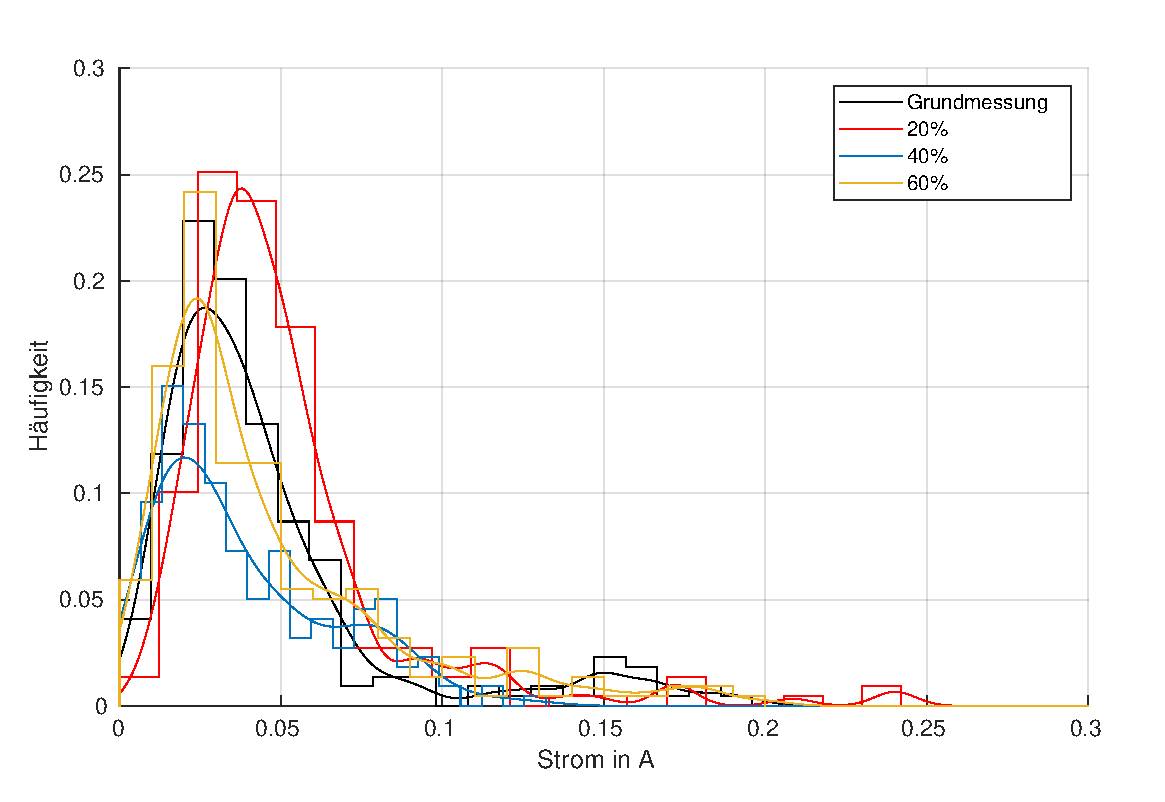
\includegraphics[width=\linewidth]{Bilder/rechts_Current_AnkleRoll_ohneM.pdf}
		\vspace{5pt}
	\end{subfigure}
	%		\hspace{20pt}
	\hfill
	\begin{subfigure}[c]{.9\linewidth}
		\centering
		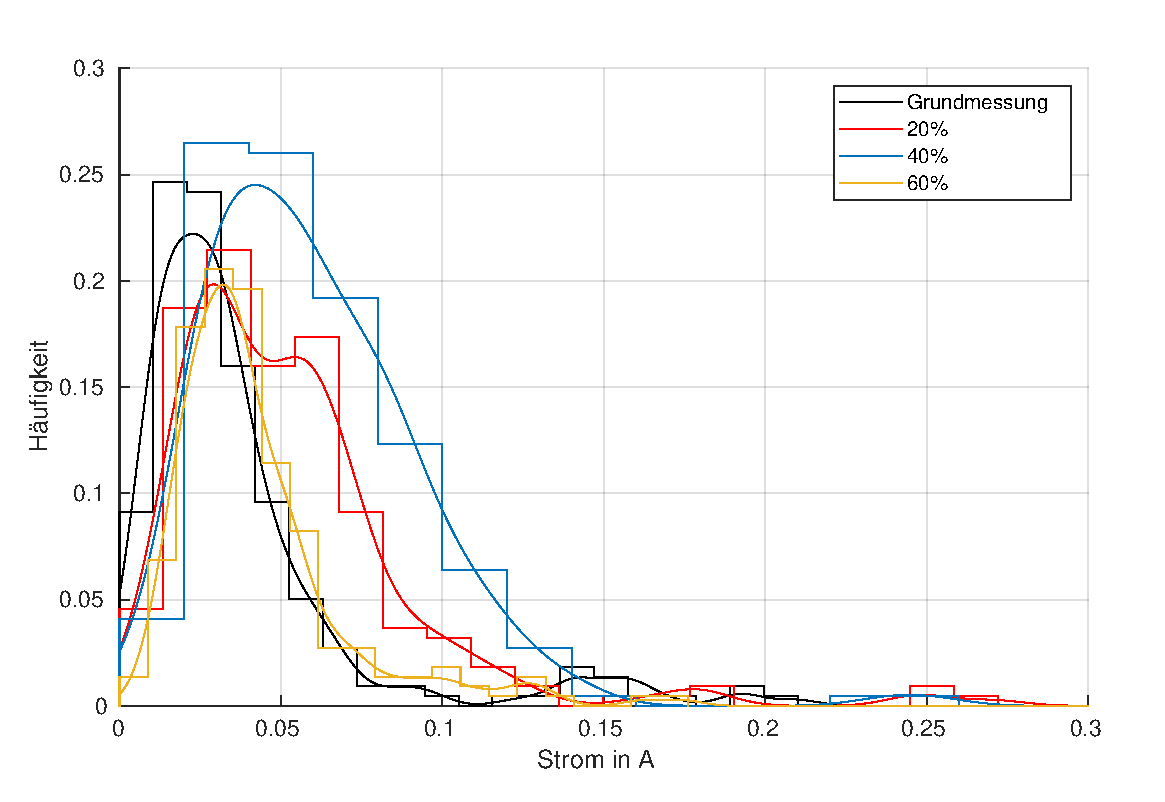
\includegraphics[width=\linewidth]{Bilder/rechts_Current_AnkleRoll_mitM.pdf}
		\vspace{5pt}
	\end{subfigure}
	%	\end{adjustwidth}
	\caption{AnkleRoll gemessener Strom im rechter Fuß, Strom in Ampère aufgetragen auf die Häufigkeit. Das Histogramm wurde ergänzt durch eine Wahrscheinlichkeitsdichtefunktion. Der obere Graph sind die Aufnahmen ohne Magneten, der untere mit Magneten.} \label{AnkleRoll_Current_rechts}
\end{figure}

% Warum genau diese Aktoren messen? -> Anziehung der Schuhe
% Warum nicht mehr aufnehmen?

% Wiederholung was der Unterschied zwischen AnklePitch und AnkleRoll ist

% Was man sieht -> keine erkennbaren Unterschiede

% Warum sieht man nichts?

% Was bedeutet das? 

% 2 Fehlschläge nicht vergessen!!!

%\subsection{Messungen von AnkleRoll zum Test}
%Die Messungen von LAnkleRoll und RAnkleRoll, zu sehen in Abb. \ref{hardware_llegjoint} und \ref{hardware_rlegjoint} wurden 20 mal wiederholt und mit den normalen Schuhen von Nao vollzogen. Dabei legte er in etwa eine Strecke von $0,8 \unit{m}$ auf der Rampe im flachen Zustand zurück. Insgesamt wurden alle verfügbaren Messwerte von AnkleRoll aufgezeichnet, das sind pro Aktor 6 Messwerte. Temperatur, Stiffness und Temperatur Status erwiesen sich als Konstant und daher nicht entscheidend, um einen Unterschied der Bodenbeschaffenheit oder Sohlen erkennen zu können. Stiffness ist immer auf $100\%$ während dem Gang. 
%Der Befehl für diesen Lauf war der moveTo() Befehl, welcher nicht weiter verändert wurde (kommt in den Theorieteil).
%
%
%In Abb. \ref{AnkleRoll_links_act} und \ref{AnkleRoll_rechts_act} sind die Messdaten von jeweils einem Fuß des Messwertes Position/Actuator abgebildet. Hier ist zu sehen, dass die Anfangswerte sich aufspalten, in positive und einmal in negative Winkelangaben. Dies ist der Tatsache geschuldet, dass die Funktion moveTo() per Zufall Nao mit dem linken oder mit dem rechten Fuß beginnen lässt. 
%
%Dies wurde für Abb. \ref{AnkleRoll_beide_act_sens_links_anfang} und \ref{AnkleRoll_beide_act_sens_rechts_anfang} sortiert. In ersterer Abbildung beginnt Nao mit dem linken Fuß. Da die Hüfte sich für den ersten Schritt nach rechts bewegen muss, verschiebt sich die Position beider Gelenke in die Negativrichtung, der Winkel wird absolut gemessen, wie in Abb \ref{hardware_llegjoint} und \ref{hardware_rlegjoint} zu sehen ist. 
%
%Außerdem sind in Abb. \ref{AnkleRoll_beide_act_sens_links_anfang} und \ref{AnkleRoll_beide_act_sens_rechts_anfang} neben den Messwerten von Position Actuator in schwarz auch die von Position Sensor in blau gezeigt. \textcolor{red}{Was diese beiden Messwerte genau unterscheidet und ob einer von moveTo() vorgegeben wird, ist noch zu entscheiden.} Der bedeutenste Unterschied ist zu Beginn der Aufnahmen. Die Position/Actuator Messung beginnt nahe 0, während Position/Sensor für den jeweiligen Fuß bei einem Wert über Null oder unter Null anfängt. 
%
%Es ist eindeutig zu erkennen, dass die Messungen erst nach der Sortierung des Anfangsschrittes ein regelmäßiges Bild ergeben. 
%
%Der Strom, welcher die Gelenke einsetzen müssen um das gewollte Ergebnis zu erzielen, scheint eine mögliche, vergleichbare Aufnahmegröße für unterschiedliche Sohlen und Umgebungen des Nao zu sein. In Abb. \ref{AnkleRoll_beide_current_links_anfang} und \ref{AnkleRoll_beide_act_sens_rechts_anfang} ist der Messwert Current aufgeteilt in Anfangsschritte gezeigt. Hier ist der Unterschied, mit welchem Fuß der erste Schritt gemacht wird, nicht so gravierend, wie bei den vorherigen Messwerten. Allerdings zeichnet sich eine Tendenz ab, dass der linke Fuß, hier in schwarz, einen höheren Strom beansprucht, als der rechte Fuß. Dies könnte dem beobachteten Fehlgang des Naos und dem zusätzlichen Geräusch bei jedem zweiten Schritt geschultet sein. Bei normaler Einstellung und ohne Korrektur würde dieser Nao einen Bogen nach rechts laufen. Um dies auszugleichen wurden bei moveTo() Anpassungen hinzugefügt.   
%
%\begin{figure}[tb]
%	\centering
%	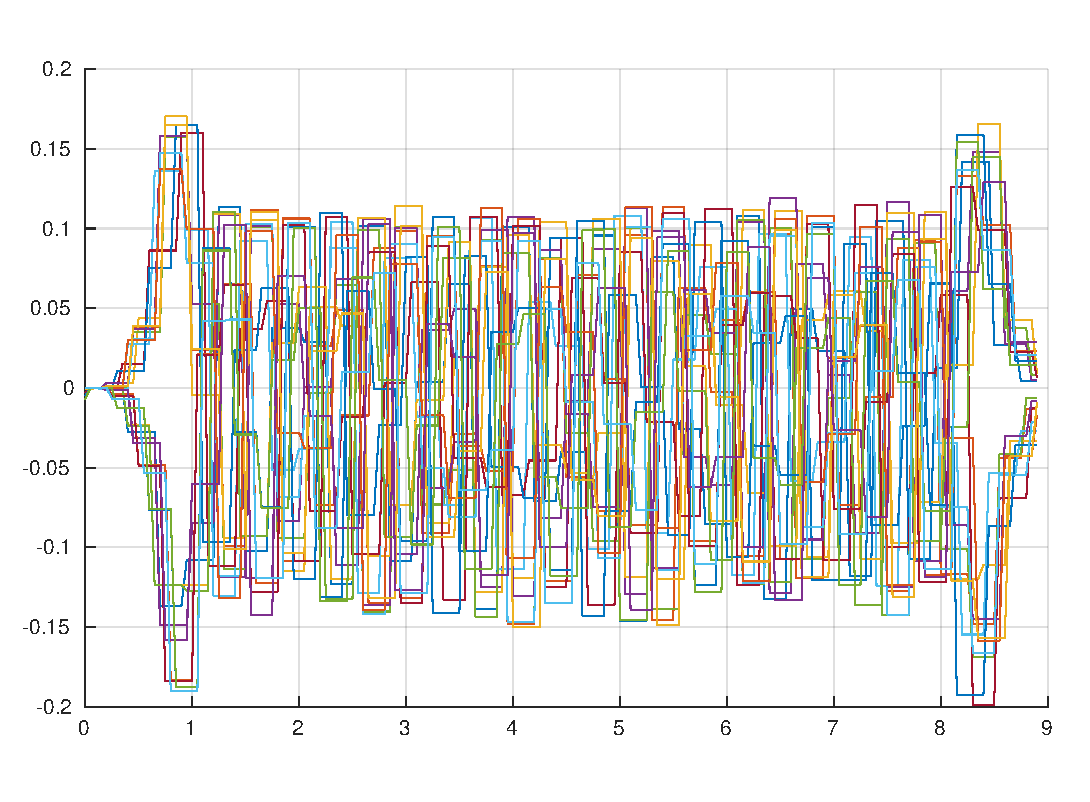
\includegraphics[width=1\linewidth]{Bilder/AnkleRoll_links_act.pdf}
%	\caption{AnkleRoll Messwert Position Actuator des linken Fußes}
%	\label{AnkleRoll_links_act}
%\end{figure}
%
%\begin{figure}[tb]
%	\centering
%	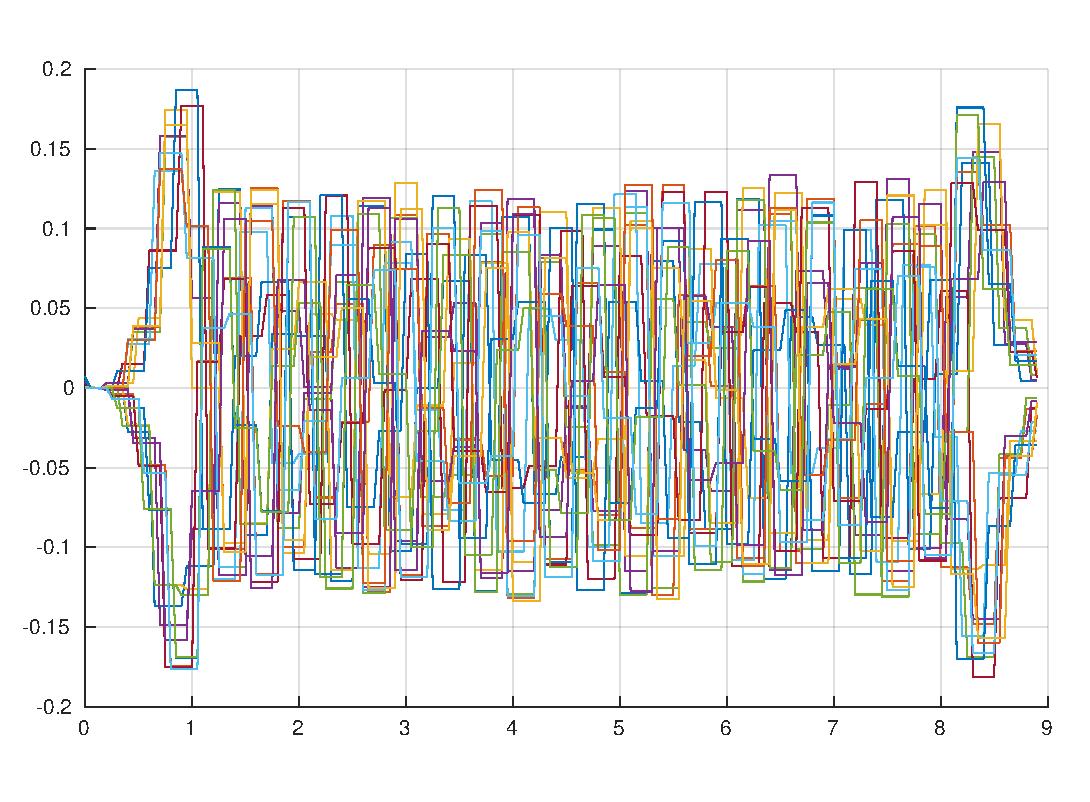
\includegraphics[width=1\linewidth]{Bilder/AnkleRoll_rechts_act.pdf}
%	\caption{AnkleRoll Messwert Position Actuator des rechten Fußes}
%	\label{AnkleRoll_rechts_act}
%\end{figure}
%\begin{figure}[tb]
%	\centering
%	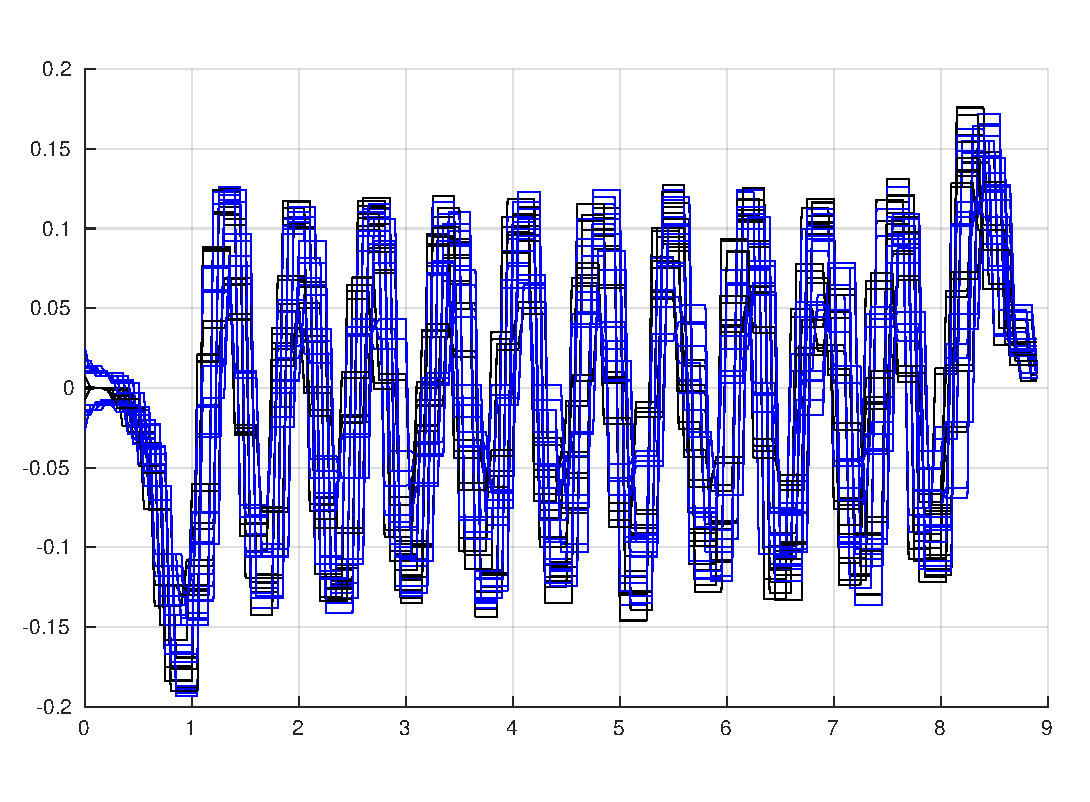
\includegraphics[width=1\linewidth]{Bilder/AnkleRoll_beide_act_sens_links_anfang.pdf}
%	\caption{AnkleRoll Aktoren beider Seiten mit dem Position/Actuator Messwert in schwarz und dem Position/Sensor Messwert in blau. Nao macht hier den ersten Schritt mit Links.}
%	\label{AnkleRoll_beide_act_sens_links_anfang}
%\end{figure}
%\begin{figure}[tb]
%	\centering
%	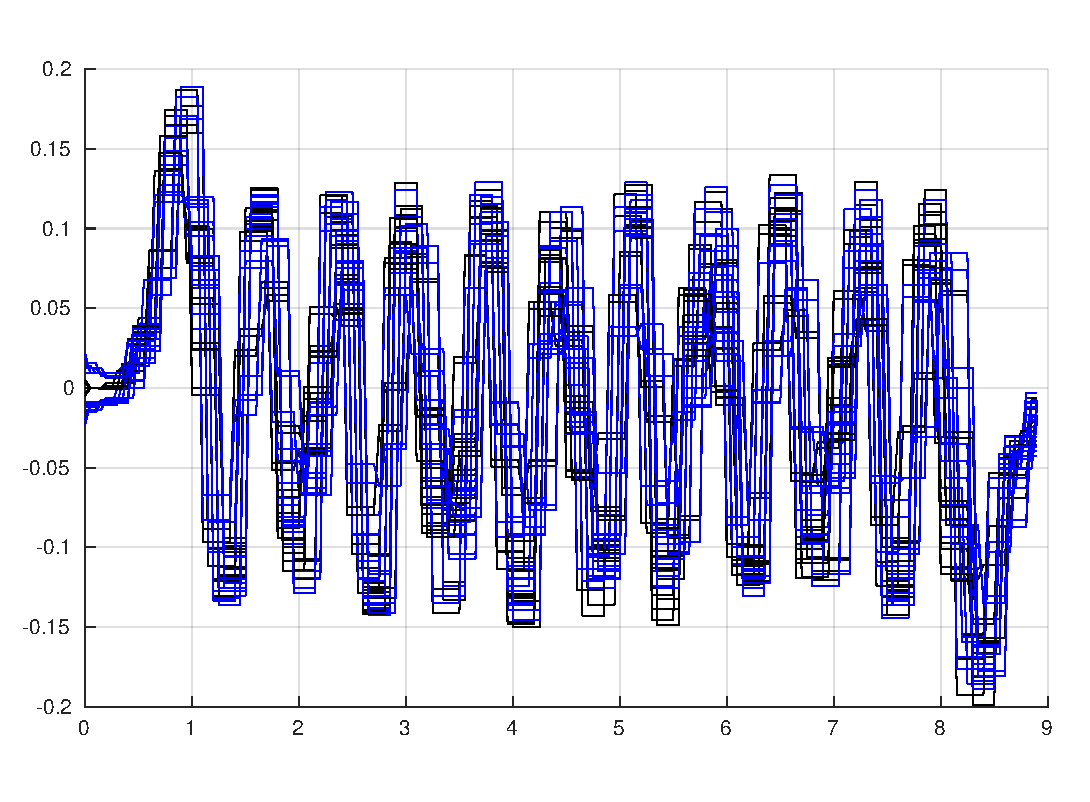
\includegraphics[width=1\linewidth]{Bilder/AnkleRoll_beide_act_sens_rechts_anfang.pdf}
%	\caption{AnkleRoll Aktoren beider Seiten mit dem Position/Actuator Messwert in schwarz und dem Position/Sensor Messwert in blau. Nao macht hier den ersten Schritt mit Rechts.}
%	\label{AnkleRoll_beide_act_sens_rechts_anfang}
%\end{figure}
%\begin{figure}[tb]
%	\centering
%	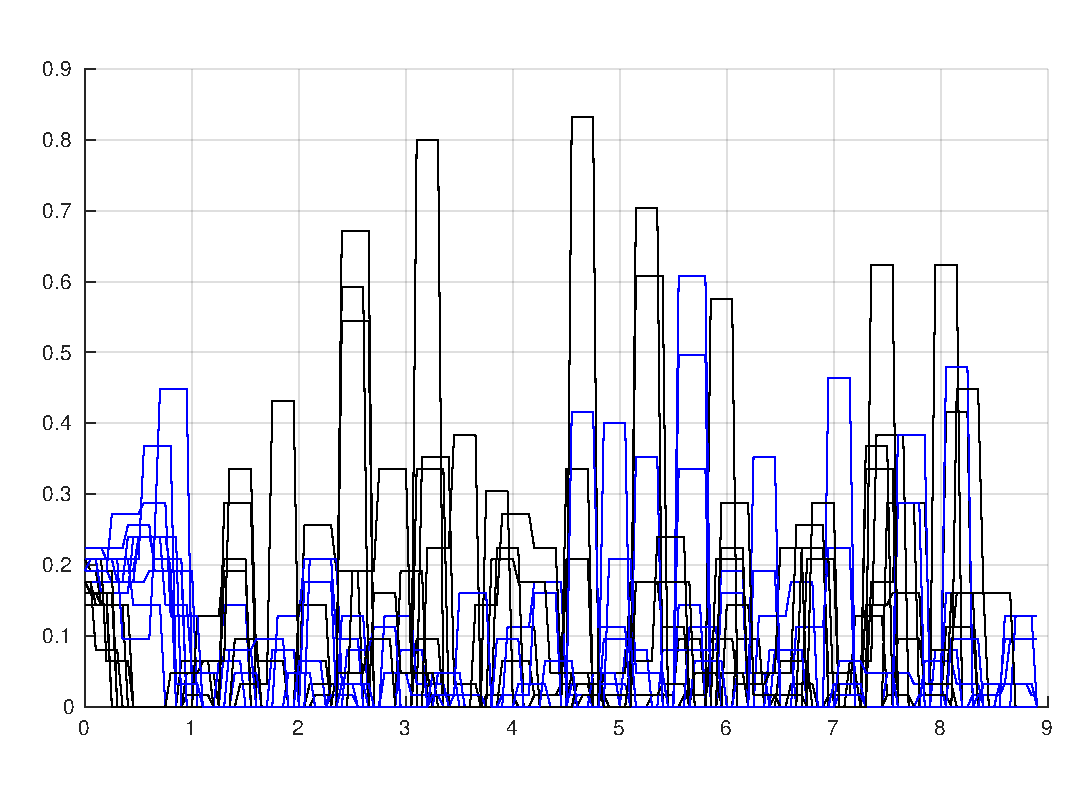
\includegraphics[width=1\linewidth]{Bilder/AnkleRoll_beide_current_links_anfang.pdf}
%	\caption{AnkleRoll Aktoren beider Seiten mit dem Current Messwert. Messwert Links ist in Schwarz, Messwert Rechts ist in Blau. Nao macht hier den ersten Schritt mit Links.}
%	\label{AnkleRoll_beide_current_links_anfang}
%\end{figure}
%\begin{figure}[tb]
%	\centering
%	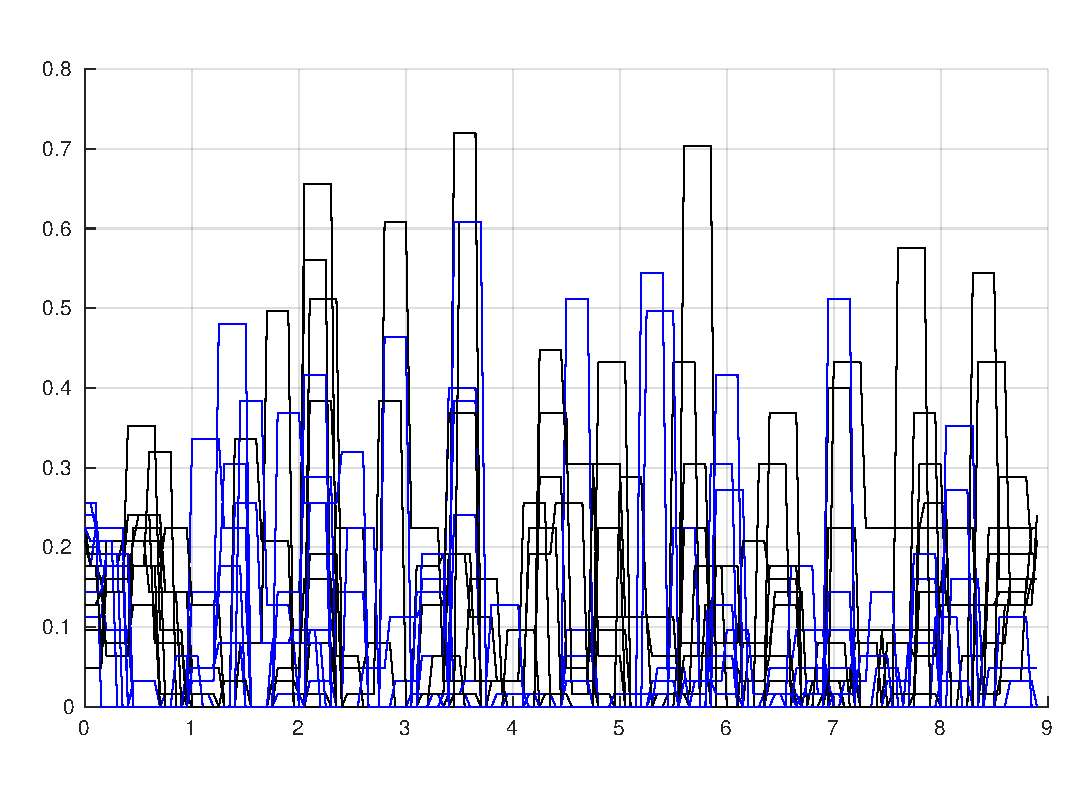
\includegraphics[width=1\linewidth]{Bilder/AnkleRoll_beide_current_rechts_anfang.pdf}
%	\caption{AnkleRoll Aktoren beider Seiten mit dem Current Messwert. Messwert Links ist in Schwarz, Messwert Rechts ist in Blau. Nao macht hier den ersten Schritt mit Rechts.}
%	\label{AnkleRoll_beide_current_rechts_anfang}
%\end{figure}

%%% Local Variables:
%%% mode: latex
%%% TeX-master: "main"
%%% End: